\chapter{Review of Literature}
\label{sec:2}
\section{Introduction}
In this Chapter, the emphasis of the discussion is on retrieval of snowpack parameters using spaceborne polarimetric SAR images. The principle and the imaging geometry of SAR system is described and a brief overview of the polarimetric SAR concepts are presented. A comprehensive exploration of all major factors affecting the SAR signal backscattered by the snow surface is discussed as available in the literature till date. 

\section{Microwave remote sensing}
Microwave remote sensing is used to study the target's characteristics using the wavelength ranging from about one centimeter to few tens of centimeters. This enables observation in all weather, day and nights without any severe restriction by rain and cloud. Microwave remote sensing in general is a function of number of observables like frequency characteristics, polarization, backscattering etc., which help to extract the physical characteristics about the targets. Microwave remote sensing is mainly classified as passive and active based on its imaging source. Passive systems uses naturally emitted, reflected or scattered microwave radiation from the Earth surface but on the other hand active systems uses its own illuminating source as shown in Figure~\ref{fig:microwave_img_sys}. Apart from SAR, microwave scatterometers and radar altimeters are the other spaceborne active microwave remote sensing sensors which have been specially launched for Ocean topography and Ocean surface wind studies respectively. The passive microwave remote sensing systems are generally radiometers.  
\begin{figure}[!htbp]
	\centering
	\includegraphics[width=0.75\columnwidth]{Figure_General/Active_RS}\\
	\includegraphics[width=0.75\columnwidth]{Figure_General/passive_RS}	
	\caption{Schematic representation of active and passive remote sensing systems.} 
	\label{fig:microwave_img_sys}
\end{figure}

SAR is an active system for imaging the Earth’s surface in day and night, in all weather, through cloud or haze and most importantly their spatial resolution is compatible with areas having high topographic variations like the Himalayan region. There are two possible operation scenarios for SAR systems viz. monostatic and bistatic. The monostatic SAR systems are equipped with both transmitting and receiving antennas in the same platform whereas in bistatic SAR system the transmitting and the receiving antennas are in separate platforms.
\section{SAR imaging geometry}
A typical SAR imaging geometry is shown in Figure~\ref{fig:SAR_geometry}. The flight direction of the satellite is called the azimuth and perpendicular to the azimuth direction when projected on to the ground is called the range. Radars can be generally classified as a real and a synthetic aperture radar based on its imaging mechanisms. In both the real and synthetic aperture radars, the range resolution is calculated by the separation of backscattered signals from various targets using the time delay between the echoes.  Doppler history is used in Synthetic aperture radar for calculation of azimuth resolution whereas angular size is used for a real aperture radar images. The SAR system focus an objects inside a beam for a longer time while traveling in the along track direction; whereby, the system synthesizes a larger antenna and produces a higher azimuth resolution.
The slant range and ground-range resolution of the SAR system is given in~(\ref{eq:range_resolution_SAR}) and~(\ref{eq:range_ground_resolution_SAR}) respectively.  
\begin{equation}
\delta R= \frac{\mbox{c}\tau}{2}=\frac{\mbox{c}}{2\beta}
\label{eq:range_resolution_SAR}
\end{equation}
\begin{equation}
\delta R_g = \frac{c\tau}{2\sin\theta}
\label{eq:range_ground_resolution_SAR}
\end{equation}
where, $\mbox{c}$ denotes the speed of light, $\tau$ is the pulse length $\beta$ is the bandwidth and $\theta$ is the incidence angle. The ground range resolution is inversely proportional to incidence angle as shown in~(\ref{eq:range_ground_resolution_SAR}). This also means that the ground range resolution in an image will be affect by the local slopes. The ground range resolution will be degraded for slopes facing towards the SAR system than the slopes facing away from the sensor. The azimuth resolution of the SAR system is given in~(\ref{eq:azimuth_resolution_SAR}), 
\begin{equation}
\delta A = \frac{L}{2}
\label{eq:azimuth_resolution_SAR}
\end{equation}
where $L$ is the antenna length. The azimuth resolution for a SAR system is only depend on the physical size of the antenna and independent of the slant range of the sensor as given in~(\ref{eq:azimuth_resolution_SAR}). Generally, smaller the antenna produces larger footprint on the surface which allows sensor to observe a longer duration of each point on the Earth surface. This means longer array can be synthesized and which allows larger Doppler bandwidth hence a finer azimuth resolution.
%\begin{figure}[!htbp]
%\centering
%\includegraphics[width=\columnwidth]{Figure_General/SAR_Geometry1.png} 
%\caption{SAR Imaging Geometry}
%%\caption*{\small(source :"Remote Sensing Illustration" by Arkarjun - Own work. Licensed under CC BY-SA 3.0 via Wikimedia Commons - \url{http://commons.wikimedia.org/wiki/File:Remote_Sensing_Illustration.jpg})}
%\label{fig:SAR_geometry}
%\end{figure}
\begin{figure}[!ht]
	\centering
	\includegraphics[width=0.6\columnwidth]{Figure_General/incidence_angle} 
	\caption{SAR Imaging geometry and incidence and local incidence angle calculation \small( accessed from "Guide to Magellan Image Interpretation" \url{http://history.nasa.gov/JPL-93-24/p46.htm} as on 19 Jan. 2016)}.
	\label{fig:SAR_geometry}
\end{figure}

\section{Basics of SAR polarimetry}

SAR polarimetry is an innovative and emerging research field which provides an opportunity to many new developments of the remote sensing applications. Several polarimetric SAR systems have been developed and flown in the space over the last few decades. Pioneers in this field such as G. W. Sinclair (1945), E.M. Kennaugh (1952), and J. R. Huynen (1970) have made significant contributions in early stage of the polarimetric radar imaging research. Soon the importance of the SAR polarimetry has increased considerably through the works of Ulaby, Fung (1990) and Alpers (1981) for their works on geophysical parameter and Ocean studies. 

Spaceborne sensors provide valuable information about the Earth's surface and environment. Active microwave sensors are of particular interest for this task due to their high resolution and their ability to image through clouds and at night. Earlier, the conventional spaceborne SAR imaging radars were implemented for long-duration missions (e.g: ERS-1 , ERS-2, JERS- 1 , Radarsat-1) which only operated in a single-frequency and a single polarization mode. The advances in technologies in the last two decades have led to the development of full-polarimetric SAR systems, where every resolution element in the image is measured as a complex scattering matrix. This complete and detailed measurements of target's polarization properties permits a much more in-depth understanding of the electromagnetic scattering process. A target which is comparable to the size of the radar wavelength strongly influence the radar backscattering. Therefore, a polarimetric sensor operating in various frequency bands provides information about the imaged target over a wide range of scales.

With the introduction of advanced radar concepts like polarimetry, interferometry and polarimetric SAR interferometry the applications utilizing SAR imagery has changed drastically. Even though, polarimetry and interferometry techniques had been demonstrated much earlier, radar polarimetry only became an operational research tool with the introduction of the NASA/JPL Airborne Synthetic Aperture Radar (AIRSAR) system in the early 1980s for Earth observation. Radar polarimetry was proven from space with the two Spaceborne Imaging Radar C-band and X-band (SIR-C/X) SAR flights on board the space shuttle Endeavor in April and October 1994. 

The time-varying direction of the EM wave, generally describe an ellipse in a plane transverse to the propagation which plays an important role in characterizing of the wave with targets and the propagation medium. This polarization transformation behavior is called as ellipsometry in optical sensing and imaging~\citep{azzam1977ellipsometry,born1970foundations,jones1941new,wolf1954optics}, it is called polarimetry (Polar: polarization, Metry: measure) in radar, lidar/ladar and SAR sensing and imaging~\citep{kennaugh1952effects,deschamps1949geometrical,rumsey1951techniques,graves1956radar,huynen1970,van1989unsupervised,zebker1987imaging,boerner1997polarimetry}. Thus, ellipsometry and polarimetry, which use the basics of the polarization of EM waves introduced in the 19th century and at the beginning of the 20th century~\citep{stokes1851composition,wiener1930generalized,born1970foundations}, are concerned with the characterization of the polarization properties of optical and radio waves respectively. 

Polarimetry research became active during the late 1940s with the introduction of dual-polarized antenna technology~\citep{kennaugh1952effects,sinclair1950transmission,rumsey1951techniques,hagfors1967study,mccormick1973method,mccormick1985optimal}. George Sinclair formulated a 2$\times$2 coherent scattering matrix to illustrate the radar target property as a polarization transformer~\citep{sinclair1950transmission}. E.M. Kennaugh also formulated a backscatter theory based on the polarizations of the 4$\times$4 scattering matrix~\citep{kennaugh1952effects}. He introduced the concept of optimal polarization by implementing the concurrent work of C. Jones, H. Mueller. Based on the original pioneering work of~\citep{kennaugh1952effects},~\citep{huynen1970} developed a phenomenological approach to radar polarimetry that had a subtle impact on the steady advancement of polarimetry~\citep{giuli1986polarization} and gave an impetus to further development, which continues today. Since the work of Huynen, important contributions have been made to the application of polarization diversity to improve the detection capability of radar systems~\citep{ioannidis1979optimum,poelman1984multinoch,swartz1988optimal}. An excellent contribution was made in the 1980s by Boerner and his coworkers through theoretical studies of the polarization properties of scattering radiation with respect to inverse scattering and target  identification~\citep{Agrawal1989,boerner1981use,boerner1991basic,boerner1993development,boerner1991basic,davidovitz1986extension,foo1984high,kostinski1986foundations}. He initiated a critical analysis of Kennaugh’s and Huynen’s work and extended Kennaugh’s optimal polarization theory~\citep{boerner1991basic}. He has been influential in causing the radar community to recognize the need of polarimetry in remote sensing applications. A new era of SAR in full polarimetry (or in quad polarization) started in 1985, with the National Aeronautics and Space Administration, Jet Propulsion Laboratory (NASA-JPL) first imaging airborne radar polarimetry~\citep{van1989unsupervised,zebker1987imaging}. The early implementations of radar polarimeters utilized conventional techniques with variable physical antenna polarization~\citep{hagfors1967study,zebker1987imaging}. The space-borne era started in 1994, when the SIR-C/X-SAR was successfully launched onboard the space shuttle.  In two short ten-day missions in April and October, 1994, SIR-C acquired SAR images of the Earth with quad polarizations at C-band (5.8 cm in wavelength) and L-band (23.5 cm in wavelength), and with single polarization at X- band. Recently, several space borne satellites like ALOS-2, TerraSAR-X, RADARSAT-2 are acquiring the SAR image with multiple polarization at their specific wavelengths.
    
SAR polarimerty is the science of acquiring, processing and analyzing the polarization state in microwave region of electromagnetic spectrum. Fully Polarimetric synthetic aperture radar, also known as quad-polarization SAR, measures a target’s reflectivity with quad-polarizations: horizontal transmitting and receiving ($\mbox{HH}$), horizontal transmitting and vertical receiving ($\mbox{HV}$), vertical transmitting and horizontal receiving ($\mbox{VH}$), and vertical transmitting and vertical receiving ($\mbox{VV}$). This is achieved by alternately transmitting horizontal (H) and vertical (V) polarization radar pulses and receiving both H and V polarizations of reflected pulses with sufficiently high pulse repetition frequencies. Unlike single or dual polarization SAR, quad-polarization data can be used to synthesize responses from any combination of transmitting and receiving polarizations. This capability provides information to characterize scattering mechanisms of various terrain covers and enhances the accuracy and details of terrain characterization~\citep{ulaby1990radar}.

The monochromatic electromagnetic plane wave propagation in time-space vector can be given based on the Maxwell equation, 
\begin{equation}
\Delta\mathbf{E}(\mathbf{r},t)-\mu\varepsilon\frac{\partial^2 \mathbf{E}(\mathbf{r}, t) }{\partial t^2}-\mu\sigma\frac{\partial \mathbf{E}(\mathbf{r}, t) }{\partial t}=-\frac{1}{\varepsilon}\frac{\partial \Delta\rho(\mathbf{r}, t) }{\partial t}
\end{equation}
where $\mathbf{E}(\mathbf{r},t)$ is wave electric field $\rho(\mathbf{r}, t)$ is volume density of free charges, $\epsilon$ and $\mu$ are permittivity and permeability of the medium. The electric field vector may be represented in the following vectorial form, 
\begin{equation}
\mathbf{E}(z,t)=
\left[\begin{array}{c}
E_{0x}\cos(\omega t-kz+\delta_{x})\\
E_{0y}\cos(\omega t-kz+\delta_{y})\\
0
\end{array}\right]
\end{equation}
\subsection{Jones vector}
The Jones vector representation of the plane monochromatic electric field aims to describe the wave polarization using the minimum amount of information~\citep{azzam1977ellipsometry,luneburg1996radar}. The time-space electric field vector can be written as,     
\begin{equation}
\mathbf{E}(z,t)=
\left[\begin{array}{c}
E_{0x}\cos(\omega t-kz+\delta_{x})\\
E_{0y}\cos(\omega t-kz+\delta_{y})\\
\end{array}\right]=Re\left\{
\left[
\begin{array}{c}
E_{0x}e^{j\delta_{x}}\\
E_{0y}e^{ j\delta_{x}}\\
\end{array}
\right]e^{-jkz}e^{j\omega t}
\right\}
\end{equation}

\subsection{Stokes Vector}

Another way of the representing the polarization of a wave that is particularly appropriate for the case of partially polarized waves is through the use of the Stokes parameters of the wave. 
\begin{equation}
\mathbf{E}\cdot\mathbf{E}^{* T} = \left[
\begin{array}{cc}
E_{x}E^{*}_{x} & E_{x}E^{*}_{y} \\
E_{y}E^{*}_{x} & E_{y}E^{*}_{y}
\end{array}
\right]
\end{equation}
For a monochromatic wave, these four parameters are defined as,
\begin{equation}
\mathbf{g}_\mathbf{E}=\left[\begin{array}{c}
g_0\\
g_1\\
g_2\\
g_3
\end{array}\right]=
\left[
\begin{array}{c}
E_{x}E^{*}_{x}+E_{y}E^{*}_{y}\\
E_{x}E^{*}_{x}-E_{y}E^{*}_{y}\\
E_{x}E^{*}_{y}+E_{y}E^{*}_{x}\\
j(E_{x}E^{*}_{y}-E_{y}E^{*}_{x})
\end{array}\right]=
\left[\begin{array}{c}
|E_x^2 +E_y^2| \\
|E_x^2 -E_y^2|\\
2Re(E_xE_y^*)\\
-2Im(E_xE_y^*)
\end{array}\right]
\end{equation}
For such a fully polarized wave, only three of the Stokes parameters are independent since,
\begin{equation}
g_0^2=g_1^2+g_2^2+g_3^2
\end{equation}
Using the relations between the ellipse orientation, ellipticity, wave amplitudes and relative phase, the Stokes parameters can also be written as
\begin{equation}
\mathbf{g}_\mathbf{E}=\left[\begin{array}{c}
g_{0}\\
g_1\\
g_2\\
g_3
\end{array}\right]=\left[\begin{array}{c}
E_{0x}^2 +E_{0y}^2\\
E_{0x}^2 -E_{0y}^2\\
2E_{0x}E_{0y}\cos\delta\\
2E_{0x}E_{0y}\sin\delta
\end{array}\right] =\left[\begin{array}{c}
A^2\\
A^2\cos(2\phi)\cos(2\tau)\\
A^2\sin(2\phi)\cos(2\tau)\\
A^2\sin(2\tau)
\end{array}\right]
\label{eq:stokes_Phi_Psi}
\end{equation}
The relations in~(\ref{eq:stokes_Phi_Psi}) lead to a simple geometric interpretation of polarization states. In the case of partially polarized waves, all four Stokes parameters are required to fully characterize the polarization state of the EM wave. In general, the Stokes parameters are related by $g_0^2 \ge g_1^2+g_2^2+g_3^2$, with equality holding only for fully polarized waves. In the extreme case of an unpolarized wave, the Stokes parameters are $g_0 > 0$ and $g_1=g_2=g_3=0$. It is always possible to describe a partially polarized wave by the sum of a fully polarized wave and an unpolarized wave.
\subsection{Wave covariance matrix}
The scattered return from the distributed targets are generally partially polarized waves, even when the illuminated signals are monochromatic with fixed frequency and polarization. This state of wave is given by the so called wave covariance matrix. The 2$\times$2 complex Hermitian positive semidefinite wave coherency matrix is also called as the Jones matrix which is defined as,   
\begin{equation}
\begin{split}
\mathbf{[J]}= \langle \mathbf{E}\cdot\mathbf{E}^{* T}\rangle=\left[\begin{array}{cc}
\langle E_{x}E^{*}_{x} \rangle & \langle E_{x}E^{*}_{y}\rangle\\
\langle E_{y}E^{*}_{x}\rangle & \langle E_{y}E^{*}_{y}\rangle
\end{array}\right]=\left[\begin{array}{cc}
\langle J_{xx}\rangle & \langle J_{xy}\rangle\\
\langle J_{xy}^*\rangle & \langle J_{yy} \rangle
\end{array}\right] \\
= \frac{1}{2} \left[\begin{array}{cc}
\langle g_0 \rangle + \langle g_1 \rangle & \langle g_2 \rangle -j \langle g_3 \rangle\\
\langle g_2 \rangle +j \langle g_3 \rangle & \langle g_0 \rangle - \langle g_1 \rangle
\end{array}\right]
\end{split}
\end{equation}
and the wave degree of polarization can be expressed in-terms of the Stokes parameters as, 
\begin{equation}
\mbox{DoP}=\frac{\sqrt{\langle g_1^2\rangle+\langle g_2^2\rangle+\langle g_3^2\rangle}}{\langle g_0\rangle}
\end{equation}
The scattered wave is completely unpolarized if $\mbox{DoP}=0$ and if $\mbox{DoP}=1$ the scattered wave is said to be completely polarized. In general, this value lies between 0 and 1 which is called as a partially polarized wave. 

The wave coherency matrix $\mathbf{[J]}$ can be written interms of the eigenvectors and eigenvalues as follows, 
\begin{equation}
\mathbf{[J]}=\bm{U_2}\left[\begin{array}{cc}
\lambda_1 & 0\\
0  & \lambda_2
\end{array}\right]
\bm{U_2^{-1}} =\lambda_1\bm{\underline{u}_1}\bm{\underline{u}_1^{T*}}+\lambda_2\bm{\underline{u}_2}\bm{\underline{u}_2^{T*}}
\end{equation}
where $\lambda_1 \ge \lambda_2 \ge 0$ are the two non-negative real eigenvalues which can be given as, 
\begin{equation}
\begin{split}
\lambda_1 = \frac{1}{2}\left\{\langle g_0\rangle+\sqrt{\langle g_1^2\rangle+\langle g_2^2\rangle+\langle g_3^2\rangle}\} \right\}\\
\lambda_2 = \frac{1}{2}\left \{\langle g_0\rangle-\sqrt{\langle g_1^2\rangle+\langle g_2^2\rangle+\langle g_3^2\rangle}\right\}
\end{split}
\end{equation}
The wave anisotropy ($A_W$) and entropy $(H_W)$ measures from the covariance matrix $\mathbf{[J]}$ also can be written as, 
\begin{equation}
A_W=\frac{\lambda_1-\lambda_2}{\lambda_1+\lambda_2} \hspace{1cm}
H_W= -\sum_{i=1}^{2}p_i\log_2p_i \hspace{0.5cm}with \hspace{0.5cm}
p_i=\frac{\lambda_i}{\lambda_1+\lambda_2}
\end{equation}  

\subsection{Target scattering vectors}\label{sec:scattering-target-vectors}
The transmitted microwave signal interacts with the Earth surface (or a target) and exhibits the changes in phase and/or the polarization state of the received signal. In the monostatic case, the transmitting and the receiving antennas are placed in the same platform. The energy that is re-radiated by the target has a response in both the vertical and the horizontal polarizations, and is expressed in the form of a 2$\times$2 scattering matrix. A fully polarimetric SAR system operating in a given frequency measures the complete scattering behavior for each pixel within an image. The backscatter alignment (BSA) convention has been the preferred system in the area of monostatic SAR polarimetry~\citep{van1990imaging,ulaby1990radar}. The $\mathbf{[S]}$ matrix, which is expressed in the BSA coordinates, is referred to as the Sinclair matrix~\citep{sinclair1950transmission,kennaugh1952effects,ulaby1990radar,zebker1991imaging,guissard1994mueller,boerner1997polarimetry} and is given in the horizontal–vertical polarization basis (H,V) as,
\begin{equation}
\mathbf{[S]}=
\left[\begin{array}{cc}
S_{HH} & S_{HV}\\
S_{VH} & S_{VV}
\end{array}\right] \hspace{0.5cm} \Rightarrow \hspace{0.5cm}
\bm{k}=V(\mathbf{[S]})=\frac{1}{2}\operatorname{Tr}(S\Psi)
\label{Eq:scattering_matrix}
\end{equation}
where each element in the matrix represents the backscatter response of the target at a specific polarization. The diagonal elements of the matrix represent the co-polarized scattering information, and the off-diagonal terms represent the cross-polarized information. In the monostatic backscattering case, the reciprocity constrains the Sinclair matrix to be symmetrical, that is $S_{XY} =S_{YX}$. The corresponding Pauli spin matrix set $\{\Psi_P\}$ and the 3-D target vectors $(\bm{k})$ can be written as, 

\begin{equation}
\{\Psi_P\}=\left\{\sqrt{2}\left[\begin{array}{cc}
1 & 0 \\
0 & 1 
\end{array} \right] \hspace{0.5cm}
\sqrt{2}\left[\begin{array}{cc}
1 & 0 \\
0 & -1
\end{array}\right] \hspace{0.5cm}
\sqrt{2}\left[\begin{array}{cc}
0 & 1 \\
1 & 0
\end{array}\right]
\right\}
\end{equation}
\begin{equation}
\bm{k}=\frac{1}{2}\left[\begin{array}{ccc}
S_{XX}+S_{YY} & S_{XX}-S_{YY} & 2S_{XY}
\end{array}
\right]^T
\end{equation}
For the Lexicographic matrix basis set $\{\Psi_L\}$and 3-D target vector $\bm{\varOmega}$ can be written as, 
\begin{equation}
\{\Psi_L\}=\left\{2\left[\begin{array}{cc}
1 & 0 \\
0 & 0 
\end{array} \right] \hspace{0.5cm}
2\sqrt{2}\left[\begin{array}{cc}
0 & 1 \\
0 & 0
\end{array}\right] \hspace{0.5cm}
2\left[\begin{array}{cc}
0 & 0 \\
0 & 1
\end{array}\right]
\right\}
\end{equation}
\begin{equation}
\bm{\varOmega}=\left[\begin{array}{ccc}
S_{XX} & \sqrt{2}S_{XY} & S_{YY}
\end{array}
\right]^T
\end{equation}
\begin{equation}
Span(\mathbf{[S]})=|\bm{k}|^2=|\bm{\varOmega}|^2= |S_{XX}|^2
+ 2|S_{XY}|^2 +|S_{YY}|^2
\end{equation}
The scattering matrix describes the information of the pure target exhibiting a particular scattering mechanism. However in general, the Earth features are more complex and produces the mixed scattering mechanism. In such a case, the information obtained from the scattering matrix is insufficient to describe the physical properties of the Earth surface. So the second order statistics of the scattering matrix i.e covariance~(\ref{Eq:Covariance_matrix}) and coherency matrix~(\ref{Eq:coherency_matrix}) are used. In this monostatic case the 3$\times$3 polarimetric coherency and covariance matrix are generated from the outer product of the associated target vector with its conjugate transpose as,

\begin{equation}
\small
\mathbf{\langle[T]\rangle}=\langle \bm{k}\cdot \bm{k^{T*}}\rangle=\frac{1}{2}\left[\begin{array}{ccc}
\langle|S_{XX}+S_{YY}|^2\rangle & \langle(S_{XX}+S_{YY})(S_{XX}-S_{YY})^*\rangle & 2\langle(S_{XX}+S_{YY})S_{XY}^*\rangle\\ 
\langle(S_{XX}-S_{YY})(S_{XX}+S_{YY})^*\rangle & \langle|S_{XX}-S_{YY}|^2\rangle & 2\langle(S_{XX}-S_{YY})S_{XY}^*\rangle \\
2\langle S_{XY}(S_{XX}+S_{YY})^*\rangle & 2\langle S_{XY}(S_{XX}-S_{YY})^*\rangle & 4\langle |S_{XY}|^2\rangle
\end{array}\right]
\label{Eq:coherency_matrix}
\end{equation}

\begin{equation}
\mathbf{\langle[C]\rangle}=\langle \bm{\varOmega}\cdot \bm{\varOmega^{T*}}\rangle=\left[\begin{array}{ccc}
\langle|S_{XX}|^2\rangle & \sqrt{2}\langle S_{XX}S_{XY}^*\rangle & \langle S_{XX}S_{YY}^*\rangle\\ 
\sqrt{2}\langle S_{XY}S_{XX}^*\rangle & 2\langle|S_{XY}|^2\rangle & \sqrt{2}\langle S_{XY}S_{YY}^*\rangle \\
\langle S_{YY}S_{XX}^*\rangle & \sqrt{2}\langle S_{YY}S_{XY}^*\rangle & \langle|S_{YY}|^2\rangle
\end{array}\right]
\label{Eq:Covariance_matrix}
\end{equation}
where the superscript $T^{*}$ denotes matrix transpose with complex conjugation and $\langle ... \rangle$ denotes a spatial or temporal ensemble average of an imaging window.  

\subsection{Polarimetric decomposition theorems}
Polarimetric target decomposition is a robust technique to characterize scattering mechanisms from polarimetric SAR data. An important objective of PolSAR decomposition technique is to extract physical information about targets from the observed scattering of microwaves. Target decomposition techniques can be broadly classified into two categories: 1) coherent target decomposition (CTD), which utilize the information contained in a target scattering matrix $\mbox{[S]}$~(\ref{Eq:scattering_matrix}) and 2) incoherent target decomposition (ICTD), which utilize the second-order statistics in terms of covariance matrices ($\mbox{[T]}$ or $\mbox{[C]}$)~(\ref{Eq:coherency_matrix},\ref{Eq:Covariance_matrix}) derived from the scattering matrix $\mbox{[S]}$. The aim of the CTD is to express the measured scattering matrix $\mbox{[S]}$ as a combination of basis matrices corresponding to canonical scattering mechanisms within a resolution cell. In which~\citep{huynen1970,krogager1990new,Cameron96,corr2002alternative} are some of the important CTD techniques. Pauli coherent target decomposition image of Radarsat-2 data over Manali-Dhundhi, India is shown in Figure~\ref{fig:Pauli_RGB_Chennai}.

\begin{figure}[!ht]
	\centering
	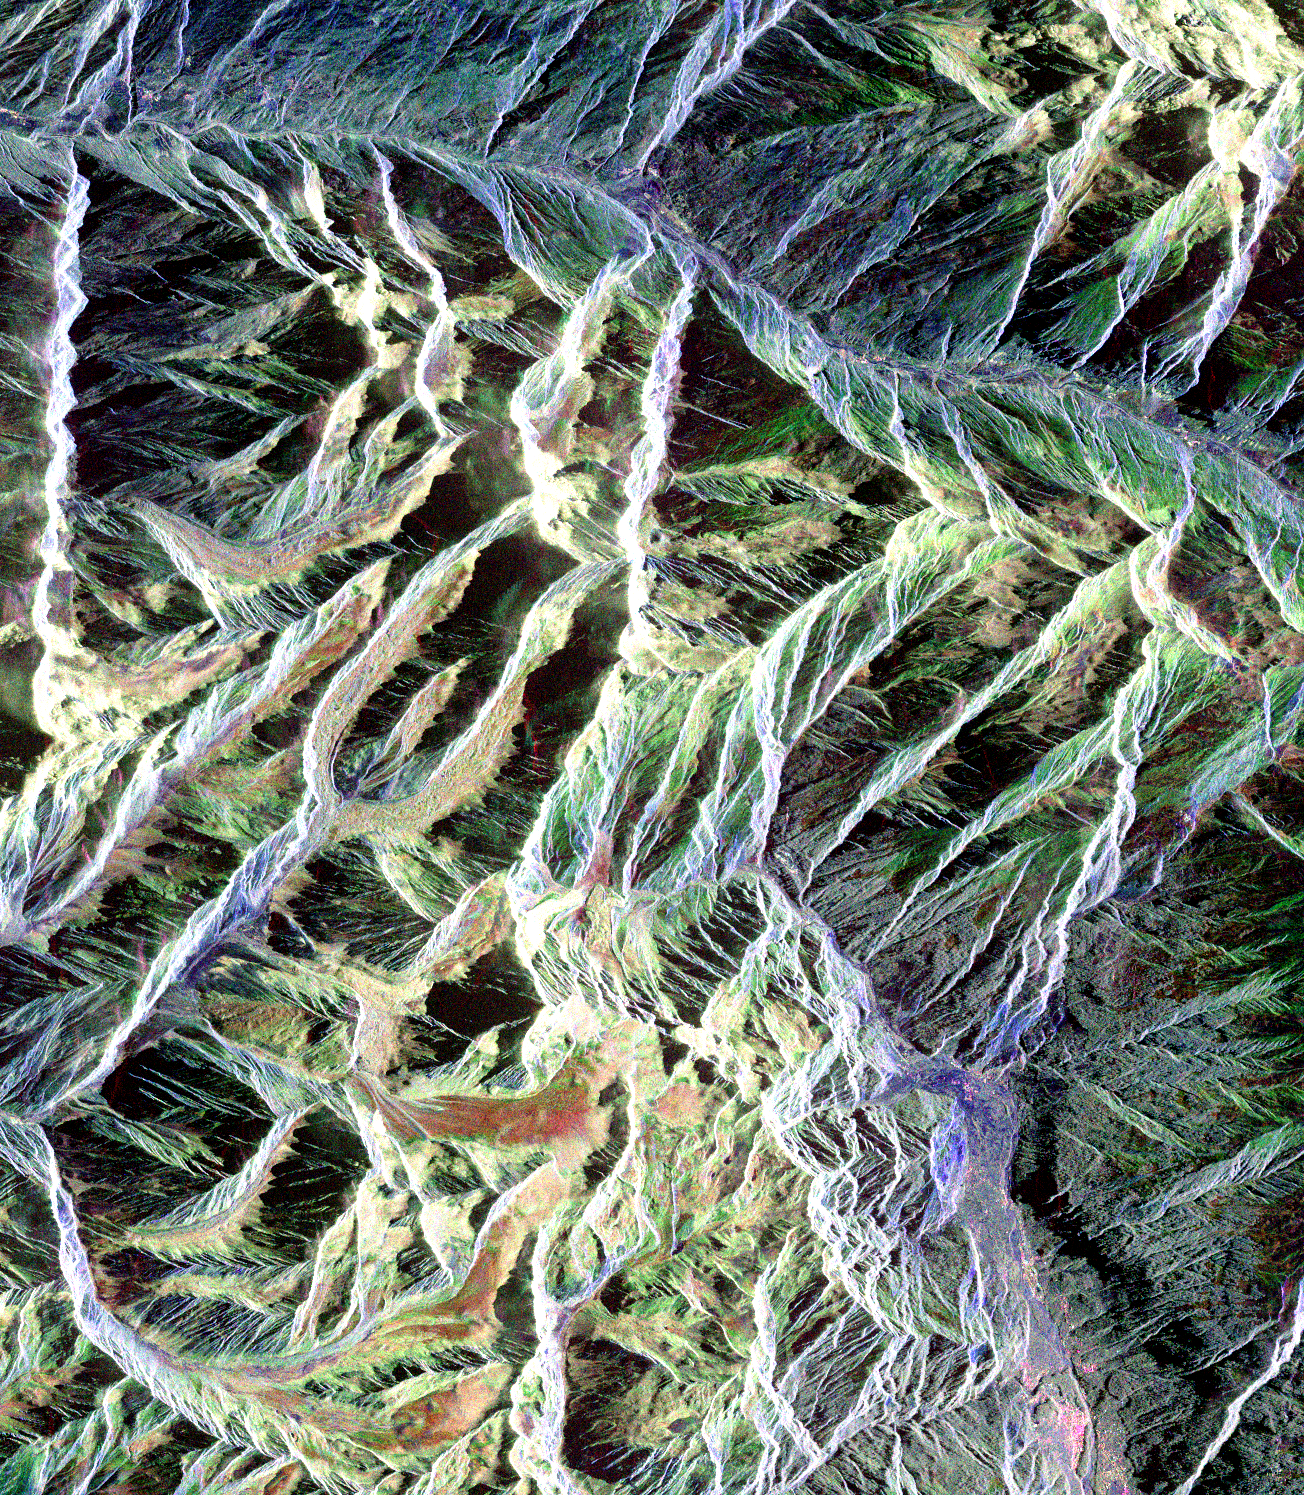
\includegraphics[width=0.6\columnwidth]{Figure_General/Manali_PauliRGB.png} 
	\caption{RADARSAT-2 Pauli RGB image of Manali-Dhundhi region,Himachal Pradesh, India}
	\label{fig:Pauli_RGB_Chennai}
\end{figure}

Furthermore, ICTD can be subdivided into eigenvalue-eigenvector-based and model-based decomposition techniques. Eigenvalue eigenvector-based decompositions provide a unique solution in terms of the scattering mechanisms~\citep{Cloude96,TOUZI2007}. These decompositions include the Von Neumann entropy ($\mbox{H}$)~\citep{john1955mathematical,cloude1986group}, the anisotropy ($\mbox{A}$)~\citep{CLOUDE97}, and the eigenvector parameters $\alpha$ and $\beta$~\citep{Cloude96,CLOUDE97}, which are assigned a physical interpretation with reference to target scattering mechanisms~\citep{cloude1986group,van1992bayesian,CLOUDE97,Cloude96}. Cloude and Pottier’s parameters have become the standard tools for target characterization and have been used as the basis for the development of new classification methods introduced for the analysis of fully polarimetric SAR data~\citep{lee1999polarimetric,pottier2000unsupervised,ferro2001unsupervised}. However,~\citep{alvarez2011coherence} raised questions regarding the assignment of each eigenvector to one of the independent scattering mechanisms by the spectral decomposition of the coherency matrix. Nonetheless, the solutions provided by model-based decompositions depend on the assumptions made about the physical scattering model. Model-based decompositions have gained considerable attention after the initial work of~\citep{freeman98}. Their decomposition assumes the target to be reflection-symmetric, i.e., the co-polarized and the cross-polarized components are always uncorrelated. This assumption was later relaxed in~\citep{Yamaguchi2005}, which included the helical scattering as a fourth component. These two decompositions are widely used in both practice and literature because of their simplicity and computational ease. Besides these, the decomposition of~\citep{arii2010general,arii2011adaptive} and~\citep{neumann2010estimation} introduced different scattering models for vegetation volume component. In~\citep{jagdhuber2013soil} this full-polarimetric decomposition with multi-angular data acquisition to estimate soil moisture from bare ground and vegetated soils have been proposed.In~\citep{cui2014complete} this a complete and an exact decomposition of the coherency matrix into a volume and two single scattering with non-negative scattering powers have been proposed. In~\citep{lee2014generalized} this the shortcomings of model-based decompositions are investigated, and suggested several models to alleviate them. Recently,~\citep{jagdhuber2014iterative} developed a hybrid model-based and eigenvalue-eigenvector based polarimetric decomposition technique with generalized volume model for soil moisture estimation under vegetation cover. 

A major advancement was made with the orientation compensation application in model-based decompositions. This was necessary because of the fact that a target with different orientations in the plane orthogonal to the radar line of sight (LOS) will have different polarimetric responses. A number of decomposition methods with orientation compensation have been proposed in~\citep{arii2011adaptive,YAMAGUCHI2011,singh13,Lee2011,An10,Chen14}. The fundamental idea behind such compensation is to minimize the cross-polarization component. The orientation compensation can, to a certain extent, reduce the overestimation of the volume power in a model-based decomposition and increase the double-bounce power. Most notably among these methods are reported in~\citep{Lee2011}, the three-component model-based decomposition by~\citep{An10}, the orientation-compensated four-component decomposition by~\citep{YAMAGUCHI2011}, and the generalized four-component decomposition by real and complex rotation of the coherency matrix by~\citep{singh13}. Most recently~\citep{bhattacharya2015adaptive} used the degree of polarization as a criteria to choose the second unitary transformation for the decomposition. The scattering powers obtained by~\cite{Yamaguchi2005} have been modified using with the concept of statistical information theory for matrices~\citep{bhattacharya2015modifying}.

\section{Factors influencing the SAR signal}
In SAR imaging, microwave portion of the EM wave signals are transmitted towards the Earth surface by an antenna. The backscattered microwave energy to the SAR system is recorded and which makes use of the conventional radar principle to form an image by utilizing the time delay. The transmitted microwave signal is scattered in all directions and the energy backscattered towards the radar is referred as radar cross-section ($\sigma$), and is a function of the amount of transmitted power absorbed and reflected by the target. The radar backscatter coefficient ($\sigma$$^\circ$) is defined as the amount of radar cross-section per unit area on the ground~\citep{jensen2000remote}. The $\sigma$$^\circ$ is a function of the wavelength, polarization, and incidence angle, as well as the target characteristics such as surface roughness, geometry and dielectric properties.

It is understood that the backscattering signal from a seasonal natural snow cover is affected by three sets of parameters: (1) snowpack parameters including snow density, free liquid water content (snow wetness), particle size and variation, characteristics of particle spatial distribution, and stratification; (2) subsurface parameters that include the dielectric and roughness properties at the snow-ground interface and (3) sensor parameters, which include the frequency, incidence geometry, and polarization;~(\cite{shi1992radar}). 

\subsection{Microwave scattering of snowpack}
The backscattering signal received by a SAR system from the snowpack is that the total sum of the surface scattering at air/snow interface, the volume scattering within the snowpack, scattering at the snow/ground interface and volume scattering from the underlying soil surface. The snow surface and volume scattering components are function of the polarization amplitude and the transmissivity respectively. Both the polarization amplitude and transmissivity depends on the dielectric constant of the medium and local incident angle. The dielectric constant of snow is primarily a function of frequency, snow wetness, temperature and density~\citep{ulaby1986microwave,hallikainen1986dielectric}. 

In case of dry snow, volume scattering is governed by dielectric discontinuities which are created by the differences in electric properties of ice crystal and air. The volume scattering increases with snow grain size and inter layering and with an increase in the amount of snow. Age of snow may influence the SAR backscatter because older snow has larger grain size than new snow grains.
The situation is totally different in the case of wet snow~\citep{ulaby1980active,stiles1980dielectric,matzler1984snow}. As soon as the top layer becomes wet (4$\%$-5$\%$ wetness by volume), the penetration capability of radar signal is reduced ~\citep{matzler1984snow}. It has been also reported in~\citep{matzler1984snow} that co-polarization ($\mbox{HH}$ and$\mbox{VV}$) backscattering coefficients of wet snow at look angle 40$^\circ$ is 10 times lower than the backscattering coefficient from dry snow and at the same time the cross polarized backscattering coefficients ($\mbox{HV}$ and $\mbox{VH}$) are 100 times lower. 

The relationship between scattering mechanism and snow wetness has been discussed in ~\citep{Shi93}. The volume scattering is inversely correlated to snow wetness. The liquid water content mainly causes an increase in snow dielectric constant which results in a significant decrease in transmission at the air/snow interface and  high dielectric loss increases the absorption coefficient. On the other hand, the surface scattering is proportional to wetness~\citep{shi1995sir}. The wavelength shift of the radar signal in snowpack was reported in~\citep{shi2000depth}. Hence, the complexity of relationship between the backscattering and snow parameters (i.e. wetness and density) makes it unrealistic to develop an empirical relationship between SAR backscattering and field measurements~\citep{singh2007envisat}. Therefore, there is need to develop inversion algorithm for snowpack parameters estimation for resolving this problem. 
  
\subsection{Influence of surface parameters} 
\begin{description}
	\item[(a) Dielectric properties:] The electrical characteristics of terrain features interact with their geometric characteristics to determine the intensity of radar returns. One measure of an object’s electrical character is the complex dielectric constant, which is a parameter that indicates the reflectivity and conductivity of various materials. The complex dielectric constant describes the ability of materials to absorb, reflect and transmit microwave energy~\citep{Campbell2002A}. Moisture content changes the electrical properties of a material, which in turn affects how the material will appear on a radar image. In~\citep{bernier1998potential} has been observed that gradual thawing of the soil caused the soil moisture and the soil dielectric constant to increase  with a resulting observed increase of backscattering signal of the snow cover. In the microwave region of the spectrum, most natural materials have a dielectric constant in the range of 3 to 8 when dry, whereas water has a dielectric constant of approximately 80. This means that the presence of moisture in soil will result in significantly greater reflectivity~\citep{ulaby1986microwave}.
\end{description}
\begin{description}
	\item[(b) Surface roughness:] The use of SAR data to retrieve surface roughness is of considerable importance in many domains, including agriculture, hydrology, and meteorology. Experimental results and studies using simulation models have shown that the radar signal is more sensitive to surface roughness at high incident angles than at low incident angles. In~\citep{holah2005potential,baghdadi2002potential,fung1994microwave,ulaby1986microwave} it has been reported that HH polarization is slightly more sensitive than VV polarization to soil surface roughness~\citep{holah2005potential}. Rough surfaces produce returns of relatively strong intensity for a wide range of depression angles~\citep{li1983tradeoffs}.
\end{description}

\subsection{Effects of SAR system parameters}  
Wavelength, polarization, incident angle and look direction are some of the important SAR system parameters. The importance of these parameters for the snowpack charaterization is presented here with more details.
\begin{description}
	\item[(a) Wavelength:] Wavelength is defined as the mean distance between two successive peak, valley or zero-crossing of a sinusoidal wave pattern and is normally measured in micrometers ($\mu\mbox{m}$) or nanometers $(\mbox{nm})$~\citep{Jensen2005introductory}. Wavelength is inversely proportional to frequency, however, When EM signal passes from one medium to another, speed of light and wavelength changes while the frequency remains the same. This wavelength interval in EM spectrum is commonly referred to as a band, channel, or region~\citep{Jensen2005introductory}. Imaging radars normally operate within a small range of wavelengths with rather broad interval. The subdivisions of the microwave region is commonly defined by $\mbox{K}_a$, $\mbox{K}$, $\mbox{K}_u$, $\mbox{X}$, $\mbox{C}$, $\mbox{S}$, $\mbox{L}$, and $\mbox{P}$ bands in ascending order of wavelength. The wavelength and the frequency range of the each band is shown in Table~\ref{table:Microwave_bands}. 	
	\begin{table}[!h]
		\caption{Microwave wavelength and frequency bands}
		\begin{tabu} to 1\textwidth { X[C] X[C] X[C]}
			\toprule
			Band & Wavelength (cm) & Frequency (GHz) \\ 
			\bottomrule
			$\mbox{K}_a$ & 0.75--1.18 & 40.0--26.5 \\ 
			$\mbox{K}$  & 1.19--1.67 & 26.5--18.0 \\
			$\mbox{K}_u$ & 1.67--2.4  & 18.0--12.5\\
			$\mbox{X}$ & 2.4--3.8   & 12.5--8.0 \\
			$\mbox{C}$  & 3.9--7.5   & 8.0--4.00 \\
			$\mbox{S}$   & 7.5--15.0  & 4.0--2.0 \\
			$\mbox{L}$  & 15.0--30.0 & 2.0--1.0\\
			$\mbox{P}$  & 30.0--100.0& 1.0-0.3\\
			\bottomrule 
		\end{tabu}
		\label{table:Microwave_bands}
	\end{table}	
	
	Radar wavelength has a fundamental influence on the interaction between the EM wave and the natural medium~\citep{garestier2006polinsar}. In principle, radar signals are capable to penetrate through the snowpack based on its wavelength and water content presents in the snowpack. In the absence of water content, penetration depth increases with the increase of wavelength~\citep{singh2009snow}. This means that longer wavelengths result in higher penetration~\citep{Campbell2002A} and could be used for mapping of wet snow~\citep{rott1993snow,nagler1996methods,shi1994snow,rao2006envisat}. The longer wavelengths are not generally useful for detecting and mapping of dry snow because snow particles are much smaller than the wavelength. It also difficult in distinguishing dry snow from bare ground using longer wavelengths SAR data. Thus, at these longer wavelengths, there is little chance for a microwave signal to be attenuated and scattered by the relatively small ice crystals comprising a snowpack~\citep{watte1970snowfield,ulaby1980active,ulaby1981microwave}. 
	
	In recent studies, it was found that the X-band image can discriminate fresh snow area from that of snow free or bare surfaces, but at C-band and L-band wavelength the signal returns may be quite similar, causing confusion in discriminating these categories. The preference of the X-band imagery with fixed channel over the C- band and L-band for general interpretation is a result of the greater sensitivity of the shorter wavelength to snow discrimination~\citep{venkataraman2008snow}. Wavelengths longer than 10–15~cm are not impeded as they move through most dry seasonal snowpacks~\citep{bernier1987microwave,bernier1998potential}. Volume scattering from a shallow, dry snow cover (SWE $<$20~cm) is undetectable at C-band (5.3~GHz, 5.6~cm), because the backscatter is dominated by soil/snow scattering. Volume scattering in dry snow results from scattering at dielectric discontinuities created by the differences in electrical properties of ice crystals and air, and by ice lenses and layers. 
		
	Atmospheric scattering is usually very small at intermediate and lower microwave frequencies and can be neglected~\citep{ulaby1980active,leconte1990preliminary,leconte1996exploring}. In case of wet snow~\citep{stiles1980dielectric,ulaby1980active,ulaby1986microwave}, when at least one layer of the snowpack (within the penetration depth of the radar signal) becomes wet (4–5~$\%$ liquid water content), the penetration depth of the radar signal is reduced to about 3–4~cm (or one wavelength at X-band)~\citep{matzler1984snow}. Thus, there may be high contrast between snow-free ground and ground covered with wet snow, thus making it possible to distinguish wet and dry snow when imaged with C-band SAR from space. Volume scattering increases with snow-grain size and internal layering, and with thickness of snow. Surface roughness is a relative concept dependent on incident microwave wavelength. 
	
	As wavelength increases, surface roughness criteria will also change. In general, more surface features will appear smoother at longer wavelengths than at shorter wavelengths. Therefore, a SAR image will appear darker in longer wavelengths than in shorter wavelengths provided the other parameters are the same~\citep{xia1997understanding}. Theoretically, azimuth resolution~(\ref{eq:azimuth_resolution_SAR}) and range resolution~(\ref{eq:range_ground_resolution_SAR}) of the SAR image is not depend on the wavelength. Therefore, wavelength will not affect the azimuth or range resolution of a SAR image. Earlier, all radar systems acquired images in a single polarization mode. Thus, relatively few studies have been carried out to examine the effect of wavelength on the detectability of snow. 
	\end{description}

\begin{description}
	\item[(b) Incidence angle:]The incidence angle is defined as the angle between the incident radar beam and the normal or vertical direction to the Earth’s surface at the point of incidence~\citep{lillesand2014remote} as shown in Figure~\ref{fig:SAR_geometry}. The look angle is defined as the angle between the vertical direction and the radar beam at the radar platform~\citep{van2011synthetic}. Depression angle is the angle between an imaginary horizontal plane and a radar beam at radar platform. Incident angle and depression angle are complementary angles, so their sum is 90$^\circ$~\citep{campbell2002introduction}. 	
		
	Radar incident angle can influence the geographical feature identification and classification to a certain degree. For low incident angle, the layover will distort the quality of SAR image in hilly terrain. For high incident angle, the radar layover is lower, but the shadow is too much, and it will lose some useful information~\citep{li2005multi}. Incident angle affects the detectability of target through its control of range resolution. On one hand, small incident angles produce poor range resolution than larger angles, as range resolution is inversely proportional to the incident angle~\citep{campbell2002introduction}. On the other hand, small incident angles provide higher spatial resolution in across track direction, improved imaging geometry in hilly and mountainous terrain (reduced foreshortening, less layover), improved thematic information content of the backscattering coefficient, and improved discrimination of small complex land cover surfaces~\citep{wegmuller2003envisat}. Experimental studies using simulation models have shown that the radar signal is more sensitive to surface roughness at high incident angles than at low incident angles~\citep{baghdadi2002potential,fung2010microwave,ulaby1986microwave,holah2005potential}.
	
	%Backscattering coefficient derived from ERS-1 data for glacier, firn and accumulation area decreases significantly at incident angle lower than 35$^\circ$ and remains almost constant between incident angle range 35$^\circ$ and 60$^\circ$. For area with vegetation and for rocks, backscattering coefficient decreases approximately linearly as incident angle increases~\citep{nagler1996methods}. For Otztal site in Alps, using ERS-1 data with low incident angle (23$^\circ$) the layover and shadow area was found 36$\%$ and 42$\%$ in ascending and descending image respectively. However, the layover area in ASAR image with swath IS6 over part of Himalayan snow cover region was found 14$\%$. The layover and foreshortening areas are more for ENVISAT swath-2 mode data which is acquired at 23$^\circ$ incidence angle. For reducing these effects, radar data at higher incidence angles (ENVISAT swath-6 or 7) are to be acquired for snow studies~\citep{singh2007envisat}.
\end{description}
	

\begin{description}
	\item[(c) Look direction: ]The direction at which the radar signal strikes the landscape, is important in both natural and man-made landscapes. In natural landscapes, look direction is especially important when terrain features display a preferential alignment. Look directions perpendicular to topographic alignment will tend to maximize radar shadow, whereas look directions parallel to topographic orientation will tend to minimize radar shadow. The extent of radar shadow depends not only upon local relief, but also upon orientations of features relative to flight path; features positioned in the near-range portion (other factors being equal) will have the smallest shadows, whereas those at the far-range edge of the image will cast larger shadows~\citep{campbell2002introduction}. Therefore it is clear that there exists a close relationship between the look direction or radar azimuth and the orientation of the topographic feature. The same type of land-cover may appear very different on a radar image due solely to a different orientation relative to the radar look direction~\citep{bryan1979effect,grey2003mapping}.
\end{description}

\begin{description}
	\item[(d) Polarization: ]Polarization is a property of certain types of waves that describes the orientation of their oscillations. The discovery of the phenomena of polarized electromagnetic energy dates back to AD 1000 when the Viking used crystals to observe the polarization of sky light under foggy condition and were able to navigate in absence of sunlight. In 1669, the first known quantitative work on light observation was published by Erasmus Bartolinus. He was followed by C. Huygens who contributed most significantly to the field of optics by proposing the wave nature of the light and discovering polarized light~\citep{lee2009polarimetric}. E.L Malus proved Newton’s conjecture that polarization is an intrinsic property of light~\citep{konnen1985polarized}. Light is a transverse electromagnetic wave. The electric and magnetic fields vibrate at right angles to the direction of propagation.  If all of the waves in a beam of light have their electric fields vibrating in the same direction, the light is described as polarized. That is, the polarization of a light wave describes the orientation of its electric field in space. Plane-polarized light has an electric field that oscillates in a specific plane perpendicular to the direction of propagation. Unlike randomly polarized light, the direction of the electric field vibration remains constant for plane-polarized light. 
	
	There are two commonly mentioned special cases of polarization, horizontal polarization, where the electric field vibrates horizontally as the wave moves forward and vertical polarization, where the electric field vibrates vertically as the wave moves forward. Plane polarized light is also called linearly-polarized light because the electric field vector can be pictured as vibrating along a line in space. If the magnitude of the electric field vector remains constant throughout each cycle, but its direction is continuously changing, the electric field can be thought of as spiraling around an axis as the wave moves forward, like the threads of an advancing screw. Elliptical polarization is the most general type of polarization. In fact, in the mathematical treatment of polarization, linear polarization and circular polarization are simply the two extremes of the elliptical case. As with circular polarization, the electric field vector rotates, but in this case the magnitude does not remain constant. That is, the tip of the electric field vector sweeps out an ellipse rather than a circle as the wave propagates.
	
	The reflected or scattered polarization characteristics of EM energy recorded by a remote sensing system can be used in many Earth resource investigations~\citep{Jensen2005introductory}. It is possible to use polarizing filters on passive remote sensing systems (e.g., aerial cameras) to record polarized light at various angles. It is also possible to selectively transmit and receive polarized energy using active remote sensing systems such as radar(e.g., horizontal transmit, vertical receive- HV; vertical transmit, horizontal receive-VH; vertical transmit, vertical receive-VV; horizontal transmit, horizontal receive-HH).
	
	Multi-polarized information about the target or Earth surface recorded by the radar system is a special interest for the bio-\ geo-physical parameter investigations. In~\citep{shi1995sir}, found that the surface and volume interaction terms are the important scattering source for cross polarized signals. The surface-volume interaction terms under the independent assumption result in an over-estimation for HH polarization. For VV polarization, however, it always over-estimates at small incident angle and under-estimates at large incidence angle. The importance of multi-frequency and multi-polarization data for separating different snow and ice regimes on glaciers and for mapping accumulation and ablation areas has been analyzed by~\citep{rott1995snow}. L- or C-band co- and cross-polarized channels in combination with X-band were found to be of main importance for snow and glacier applications. Multi-polarized, multi-frequency microwave data can suffice the needs up to some extent when a simplified form of Integral Equation Method (IEM) is used. 
	
	The single band (C-band) SAR data is inadequate for the estimation of snow wetness because which takes more than one unknown parameter into consideration. The effect of the snow volume scattering albedo and surface roughness can be minimized to estimate the snow parameters using multi-polarization(dual polarization) backscattering coefficient (HH, VV and Re{[\mbox{HHVV}]}) measurement~\citep{Shi95wetness}. In~\citep{autret1989theoretical} and ~\citep{chen1995simple} also have reported that the influence of surface roughness can be minimized using the co-polarized ratio (HH/VV). Hence, multiple polarizations helps to distinguish the physical structure of the scattering surfaces. Co-polarization signals are dominated component for surface scattering eg., $\mbox{VV}$ polarization and cross-polarization is the dominant component for volume scattering eg.,$\mbox{VH}$ polarization.
	
	By comparing both the $\mbox{HH}$ and $\mbox{HV}$ images, the features and areas that represent regions on the landscape that tend to depolarize the signal can be identified. Such areas will reflect the incident horizontally polarized signal back to antenna as vertically polarized energy- that is they change the polarization of the incident microwave energy. Such areas can be identified as bright regions on the $\mbox{HV}$ image and as dark or dark grey regions on the corresponding HH image. The polarization of the energy that would have contributed to the brightness of the $\mbox{HH}$ image has been changed, so it creates instead a bright area on the HV image. The same information can be restated in a different way. A surface that is an ineffective depolarizer will tend to scatter energy in the same polarization in which it was transmitted; such areas will appear bright in the HH image and dark on the HV image ~\citep{campbell2002introduction}. The alternating polarization mode of ASAR is capable of providing multi-polarimetric acquisitions by means of SAR acquisitions, where switching is made on polarizations instead of sub swaths. Each of these polarizing channels have varying sensitivities to different surface characteristics and properties. For example, the dynamic range of the like polarized component is larger than that of the cross-polarized component for snow cover area~\citep{shi1997estimation}; this is in contrast to the measurement for forested areas, where the dynamic range of the cross-polarized component is larger than that of the like-polarized component~\citep{dong1997radar}. 
	
	The information from alternative polarization of SAR images are the great importance in the process of identification and classification of different types of scattering mechanisms, and where the penetration depth is different at different polarization channels. However, use of satellite SAR polarimetry data sets for snow cover area analysis is only a beginning and there are still many unknowns. Given the paucity of data analysis of snow covered area with multi-polarized data sets and the variation in the earlier results much remains to be determined about the exact relationships between snow parameters and radar backscatter. In~\citep{venkataraman2008snow}  have reported that the backscattering coefficient value of $\mbox{HH}$ polarization is lower than the $\mbox{VV}$ polarization while studying the snow wetness in the Himalayan snow covered region. 
\end{description}
\subsection{Snowpack parameters}
\label{sec:2.3}
Microwave signal interaction with targets (e.g. snow) changes mainly according to the frequency (or wavelength) and the polarization. The interaction depends on the shape and orientation of the scatters and the scattering mechanisms (i.e. whether it is single or multiple scattering). The polarization characteristics get vary for different polarization channels for the same target. By using imaging radar, the polarimetric characteristic can be measured for each pixel to understand the scattering mechanism associated with it. The geophysical information associated with the scattering mechanism could be inferred from these polarimetric responses. Generally, single frequency and single polarization radar techniques have a considerable degree of ambiguity for different types of targets. To overcome this, the dimensionality of the observation needs to be increased. This can be achieved through the use of multi-frequency and/or multi-polarization radar systems. Multi-temporal and multiple incident angles are other ways of increasing the dimensionality of observation. In this section important estimation of snowpack parameters (wetness and density) relative to the proposed objectives and their characteristics is discussed through the available literatures. Exhaustive review of mountainous snow cover properties using active microwave remote sensing is presented in~\citep{snehmani2015review}.

\begin{description}
	\item[(a) Snow wetness: ] Snow wetness is a percentage of free liquid water presented in the snowpack. This is an useful indicator for the prediction of snow melt start and runoff and also a important parameter for the prediction of avalanches, flooding, global warming, and climate change. Estimating snow wetness requires a good understanding on the scattering mechanism of wet snow. This is a very complex task due to the highly variable physical structure of wet snow. Effective permittivity of snowpack is highly depended on the presence of water droplets or particles in it. For dry snowpack, the backscatter contribution from the air-snow surface is small and thus can be neglected. So, the total backscatter contribution is a combination of snow volume and snow-ground surface only~\citep{Shi2000}. 
	
	For dry snow, the penetration depth, $\delta_p\approx$ 10~m at 10~GHz and decreases to 1~m at 40~GHz~\citep{Rott85}. Volume scattering in snow is due to dielectric discontinuities. Volume scattering from thin dry snow cover is undetectable at wavelengths longer than 10 or 15 cm, however, the level of scattering is dependent on the amount of snow on the ground (more snow implies more dielectric discontinuities for scattering)~\citep{bernier1987microwave}. The extinction coefficient, $\kappa_e$ which is inversely related to $\delta_p$ is equal to the sum of the absorption coefficient ($\kappa_{a}$) and scattering coefficient ($\kappa_{s}$). For wet snow, $\kappa_{e}\approx\kappa_{a}$, at microwave frequencies as the absorption losses are much larger than the scattering losses. Due to this, $\delta_p$ is of the order of 1 or 2 wavelengths and hence, the snow-ground scattering may be neglected. For C-band SAR, the backscattering signal from wet snow is dominated by the scattering from air-snow interface and snow volume medium~\citep{Shi95wetness}.
	SAR backscattering coefficient is sensitive to many snow parameters that hydrologist use, especially free liquid water content in the snowpack because of the large dielectric contrast between ice and water in microwave spectrum (~\citep{Shi93}. Several investigators~\citep{Arslan05,shi1992radar,shi1997estimation,Shi95wetness,strozzi1999mapping,Singh2007_spie,singh2010snow} reported that backscatter coefficient image of radar is extremely useful for the quantitative estimation of snow wetness (percentage of liquid water content in snowpack).
	 
	L band, horizontal polarization SAR shows that the backscattering coefficient ($\sigma^0$) decreases with increase in snow depth and snow wetness for a given snow density and surface roughness.  The variation in grain size does not seem to affect this relation.  In case of dry snow, there is very little change in $\sigma^0$ with change in snow depth.  Using this relation, it may be possible to derive snow wetness from backscatter coefficient if we know the snow depth.  However, it is not credible to derive a simple empirical relation between snow wetness and radar backscattering, as previous investigations have shown both negative and positive relationships between backscattering coefficients and snow wetness~\citep{Shi95wetness}. This relationship is complicated, as surface roughness affects this relationship. Surface roughness affects the relationship between the backscattering coefficients and snow wetness.  For low wetness ($\le 3\%$) the dielectric contrast between air and snow is small and volume scattering dominates, so backscattering is now sensitive to surface roughness and decreases as wetness increases.  However, for wetter snow, backscattering becomes sensitive to surface roughness, because the surface-scattering component increases while the volume-scattering component decreases. Thus the relationship between backscattering and snow wetness is controlled by the scattering mechanism.  When the surface is smooth, volume scattering is the dominant scattering source. 
	
    As snow wetness increases, both the volume scattering albedo and the transmission coefficients greatly decrease.  This results in a negative correlation between the backscattering signals and snow wetness.  When the surface is rough, increasing snow wetness results in greatly increased surface scattering interaction and surface scattering becomes the dominant scattering process.  Therefore, a positive correlation between the backscattering signals and snow wetness will be observed~\citep{Shi93}. Moreover, the relationship between co polarization and snow wetness can be either positive or negative, depending on snow characteristics, surface roughness and incidence angle. In~\citep{Singh2007_spie}, an empirical model has been developed for the estimation of snow wetness using $\mbox{HH}$ polarization backscattering coefficient. It has been observed that, the backscattering coefficient is approximately constant for the snow wetness values ranges from 3.0$\%$ - 5.0 $\%$.  This complexity of the relationship between the backscattering coefficient and snow wetness makes it unrealistic to develop a simple empirical relation. 
		
	A inversion model has been developed for the estimation of snow wetness based on Small Perturbation Model (SPM)~\citep{Shi93}. This model is applicable for the incidence angle ranges from 15$^\circ$-70$^\circ$ and for the small to moderate surface roughness variations. Further,~\citep{Shi95wetness} used fully polarimetric space shuttle borne SIR-C data to derive snow wetness by inverting a first order backscatter model (surface and volume scattering). By measuring three components ($\sigma_{vv}^0$= Backscattering Coefficient (BSC) of VV polarization, $\sigma_{hh}^0$ = BSC of HH polarization and $\sigma_{vvhh}^0$=$Re[VVHH^*]$) they were able to minimize effects from volume scattering and surface roughness (i.e. reduce the dimensionality of inversion problem) to estimate snow permittivity, which subsequently is related to snow wetness.~\citep{singh2006snow} also developed dielectric retrieval algorithm using first order surface scattering and volume scattering based on Physical Optics Model (POM). Further the dielectric constant has been related to snow wetness. Absolute error between Envisat-ASAR estimated and field measured value was observed to be 2.52$\%$ by volume.
	
	~\citep{Kendra98} conducted experiments to measure radar backscatter at C and X band of artificial snow of varying depths. The results of this study are amenable to comparison with predictions based on theoretical methods for modeling volume scattering media.  A direct polarimetric inversion approach has been described through which the characteristics of the snow medium are extracted from the measured data.~\citep{Kendra98} have also collected backscatter values alongwith concurrent snow liquid water content (wetness) measurements in experimental snowpacks. These measurements were used to confirm the validity of the algorithm developed by~\citep{Shi95wetness} for the retrieval of snow liquid water content. It has been found that the algorithm was able to precisely characterize the snowpacks for their wetness.~\citep{niang2007new} also developed statistical inversion model which performs retrieval of the snow wetness using ENVISAT- ASAR alternating polarization data.~\citep{Shi95wetness} model required fully polarimetric SAR data, but ENVISAT-ASAR has capability of data acquisition in dual polarization only. Hence,~\citep{singh2010snow} modified~\citep{Shi95wetness} snow wetness algorithm for dual polarization and the modified algorithm was implemented on ENVISAT-ASAR dual polarization data.  Model estimated wetness was found to be quite in agreement with measured wetness with 2.8$\%$ absolute error.	
\end{description}

\begin{description}
	\item[(b) Snow density: ] In general, snow is electromagnetically a three component dielectric mixture of ice, water and air. Dry snow is an inhomogeneous medium consisting of ice particles and air voids, whereas wet snow consists of ice spheres embedded in an air-water medium. Snow density is an important parameter of the snowpack which influences the thermal, mechanical and optical properties of snow layers. It is thus a vital parameter for avalanche prediction~\citep{hirashima2009adjustment,brun1989investigation} and snow hydrology~\citep{rango1995revisiting,jonas2009estimating,sturm2010estimating}. The snow density is a complex parameter that can vary spatially, temporally and vertically within the snowpack profile~\citep{bormann2013spatial}. Wind erosion, melt-refreeze events, compaction and snow metamorphisms acting in response to internal temperature and moisture gradients~\citep{sommerfeld1970classification,colbeck1982overview} are responsible for seasonal snowpack densification. The snow particles get reshaped into sphere-like structures due to wind erosion. These sphere shaped particles, then closely pack together thereby increasing the density. The melt-freeze processes~\citep{colbeck1982overview} due to temperature fluctuations is majorly responsible for snow densification. The liquid water content present in the snowpack~\citep{brun1989energy,marshall1999snow} along with the destructive snow metamorphisms occurring when vertical temperature gradients are weak~\citep{colbeck1982overview} results in smaller and rounded particles. Bulk weight density of snow according to EN 1991-1-3 and NS 3491-3 (settled snow is measured several hours or days after its fall; old snow several weeks or months after its fall). 	As given in NS 3491-3 and EN 1991-1-3 (European Committee for Standardization, 2003) the mean density of snow is given in~Table~\ref{table:mean_density_of_snow}~\citep{MET40}.
	
	\begin{table}[!htbp]
		\caption{Mean density of different snow types}
		\centering
		\begin{tabu} to 0.8\textwidth { X[l] X[r]}
			\toprule
			Type of snow & Bulk weight density (kg m $^{-3}$) \\ 
			\bottomrule
		\end{tabu}
		\begin{tabu} to 0.8\textwidth { X[l] X[r]}
			Fresh & 100 \\ 
			Settled & 200\\ 
			Old & 250-350\\
			Wet & 400 \\
			\bottomrule
		\end{tabu}
		\label{table:mean_density_of_snow}
	\end{table}
	
	Several works have been done with the microwave interaction of snow at various frequencies~\citep{stiles1980active,ulaby1980active,ulaby1984snowcover,rott1987possibilities,rott1988study}The radar backscattering coefficient is a function of various parameters classified as surface parameters and radar observation parameters. The radar observation parameters include the transmission wave frequency, polarization, and incidence angle. Surface parameters include roughness, geometrical shape and dielectric properties of the target. SAR data showed its potential for snow cover monitoring in the boreal forest zone~\citep{koskinen1997use}. Several theoretical models have been developed and experimental data sets have been analyzed to relate backscattered coefficient of snow covered terrain with its physical properties~\citep{Shi95wetness,Shi2000,shi2000depth,besic2012dry,besic2015stochastic}. All these studies have indicated that the factors which have been found to have the most profound influence on the backscatter coefficient are snow water equivalent, liquid water content and moisture content of soil. The snow surface roughness and size distribution of ice crystals are also some of the important factors and the extent of their importance is further dependent on the wavelength used and the angle of incidence. Satellite remote sensing is a key tool in monitoring the snow pack parameters over a large area. Microwave remote sensing measurements can be efficiently used to infer bulk properties of snowpack. 
	
	Many algorithms have been developed for SAR data to estimate the snow dielectric constant~\citep{Shi93,Shi95,Singh2007_spie,niang2007new,singh2010snow,surendar2013improved,bhattacharya2014snow}. The real part of the relative dielectric constant~($\varepsilon{'}$) is solely dependent on the density. An inversion approach for the estimation of snow density from full polarimetric SAR data was developed by~\citep{Shi2000} using L-band data from SIR-C/XSAR mission. This algorithm does not require a priori knowledge of the subsurface dielectric and roughness properties and it can be applied over a large range of incident angles (10$^\circ$-70$^\circ$). The estimated snow density compared to field measurements shows an RMSE of 0.042 gcm$^{-3}$ and a relative error of 13$\%$. However, this method cannot be applied where the subsurface is dominated by volume scattering, as may be the case with snow-covered firn. Even though they used full polarimetry data, they did not utilize the complete full-polarimetric information. However, they have only considered a first order backscattering coefficients to invert snow density. There are many snow and glacier studies done over the Indian Himalayan region using fully polarimetric SAR  data~\citep{singh2011a,singh2012a,singh2012b,singh2014a,singh2014b}. Dry snow density estimation algorithm over the Indian Himalayan region was proposed in~\citep{Snehmani2010density}. In this, C-band ENVISAT-ASAR data has been used and snowpack volume and snow-ground scattering components were considered for the inversion. Very recently,~\citep{surendar2015density} demonstrated and validated the snow wetness and density estimation algorithms based on full polarimetric C-band Radarsat-2 data over Indian Himalayan region. The snow density algorithm accounted for only a snowpack volume scattering for the C-band data. 
	 
\end{description}
	
\section{Current PolSAR reserch for snowpack parameter studies}
	Recently, some ad-hoc programmes initiated to study the global snow cover to understand the fresh water storage. In particular, the ESA’s Cold Regions Hydrology high-resolution Observatory (CoReH2O) mission offers many researchers to carried out the study on snow parameters estimation. Some SAR sensors onboard Unmanned Aerial Vehicle (UAV) (Ex., snowSAR) was also flown to study the snowpack characterization with high amount of accuracy. The availability of high spatial temporal resolution and multi-polarization $\&$ multi-frequency SAR systems provide an opportunity to researchers to explore more precise snowpack information. A new empirical relationship has been developed for the estimation of SWE using X-band COSMO SkyMed $\mbox{VV}$ polarization data~\citep{Pettinato2013}. This empirical relationship may be highly depends on the study area and data acquisition time and weather conditions. This method is also valid only for dry snow cover with the snow depth in the range of 60-70cm. 
	
	
	Rott et al. (2014) and Macelloni et al. (2014) used the minimization approach to estimate the SWE over the terrain and forest cover area respectively using multi-frequency dual polarization SnowSAR data. This methods need priori information to apply the minimization and retrieve SWE and this methods are applicable only for dry snow cover. Leinss et al. (2014 (a)) estimated the fresh snow depth using co-polarization phase difference of X-band SAR data.  They have presented the relationship between the microstructure of snow and the co-polarization phase difference and have also studied the variation of CPD with respect to the temperature gradient.  Leinss et al. (2014 (b)) have also presented an approach for estimation of SWE using differential interferometry technique. They have derived a linear function between the SWE and the phase difference for dry snow using Ku and X band SnowScat instrument. Very recently, Surendar et al. (2015 (a), 2015 (b)) demonstrated and validated the snow wetness and density estimation algorithms based on full polarimetric C-band Radarsat-2 data over Indian Himalayan region. The snow density algorithm accounted for only a snowpack volume scattering for the C-band data. Further this algorithm can be modified and suitably used for higher wavelength bands and for complete dry snowpack conditions. 
	